\documentclass[12pt]{article}
\usepackage[a4paper, margin=.30in]{geometry}
\usepackage{graphicx ,
            wrapfig,
            xcolor, 
            enumerate,
            amsmath,fontenc,tcolorbox
            }
\usepackage[european, straightvoltages,EFvoltages]{circuitikz}
\newcommand\headerMe[2]{\noindent{}#1\hfill#2}
\renewcommand{\thesection}{\Roman{section}}

\title{Leçon : }
\author{Zakaria HAOUZAN}
\date{\today}

\begin{document}
% headers --------------
\headerMe{Matière : Physique-Chimie}{Professeur : Zakaria HAOUZAN}\\
\headerMe{Unité : La Mécanique}{Établissement : Lycée SKHOR qualifiant}\\
\headerMe{Niveau : TCS}{Heure : 2H}\\

% ------Content ________
\begin{center}
  \Large{Leçon $N^{\circ}11$: \color{red} Caractéristiques de quelques dipôles passifs }
\end{center}

\section{Dipôles passifs: }

\subsection{Définition:}
Un dipôle est un composant électronique possédant deux bornes.

La caractéristique d'un dipole est définit comme la fonction qui relie la tension U entre ses bornes et l'intensité I du courant qui le traverse : U=f(I) ou I=f(U).

Le dipole est dit passif si sa caractéristique passe par l'origine

Exemples de quelques dipoles passifs : le conducteur ohmique ,la lampe , la diode ...

%\begin{wrapfigure}[4]{r}{0.39\textwidth}
    %\vspace{-1cm}
%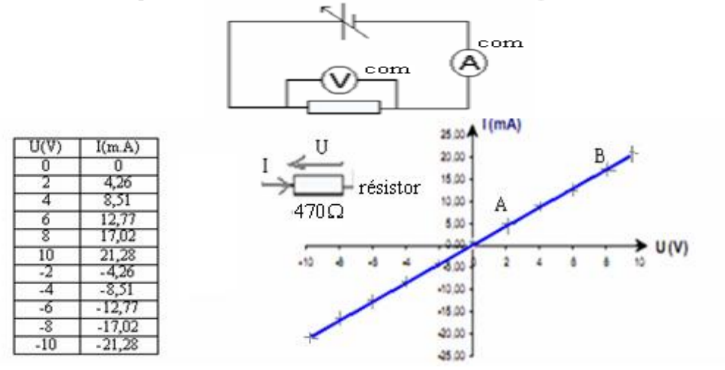
\includegraphics[width=0.39\textwidth]{./img/caracteristique_Resistor.png}
%\end{wrapfigure}


\subsection{Convention récepteur: }
Dans la convention récepteur la tension U aux bornes d'un dipôle passif et l'intensité I du courant qui le traverse
sont de sens contraires.

\begin{center}
  \begin{circuitikz}[european resistors]
      \draw (-0.5,0.1)node{A} (0,0)to[R,v<=$U_AB$,i=I, name=D] (2,0);
      \draw (2.2, 0) node{B};
    
  \end{circuitikz}
  \end{center}

\section{Caractéristiques de quelques dipôles passifs }
\subsection{ Montage expérimental:}
Pour tracer la caractéristique d'un dipôle D on utilise l'un des deux montages suivants:


\begin{center}
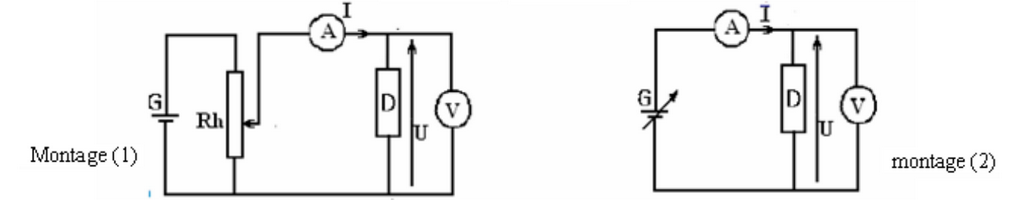
\includegraphics[width=0.5\textwidth]{./img/Tension_exper.png}
\end{center}
\subsection{Caractéristique d'une lampe à incandessance:}
On réalise le montage (2) en utilisant comme dipôle une lampe à incandessance :

\begin{center}
  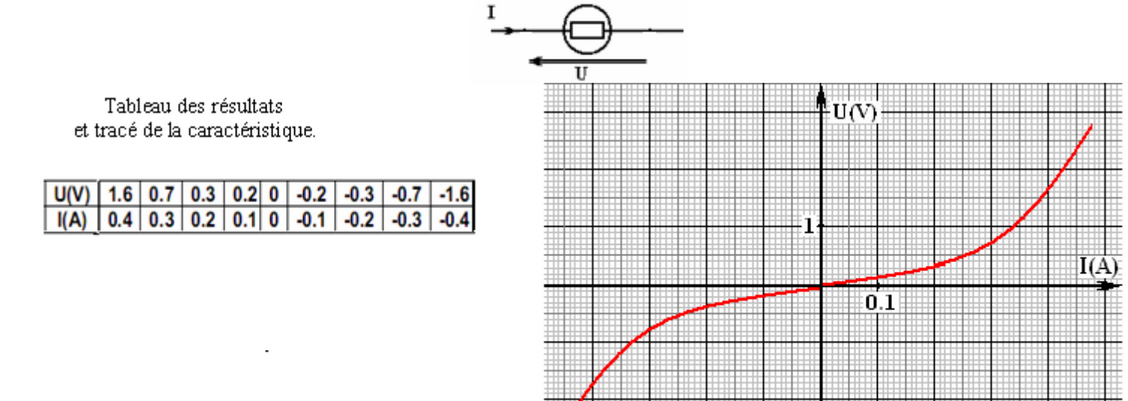
\includegraphics[width=0.9\textwidth]{./img/lampe_U.png}
\end{center}

\begin{tcolorbox}{}
La caractéristique est non linéaire et elle passe par l'origine , donc la lampe à incandessance est un dipôle passif.
La caractéristique est symétrique donc les deux bornes de la lampe jouent le même rôle.
\end{tcolorbox}

\subsection{Caractéristique d'une diode normale: }
La diode normale est constituée d'un semi-conducteur: le silicium ou le germanium dopé .

Le dopage est l'introduction dans le semi-conducteur de très faibles quantités d'un corps étranger appelé dopeur.

Pour les semi-conducteurs (Ge ou Si ) , les dopeurs sont: soit l'Arsenic (As) ou le phosphore (P) ........

Ces dopeurs sont introduits très faible dose ( de l'ordre de 1 atome du dopeur pour $10^6$ atomes du semi-conducteur


\begin{center}
  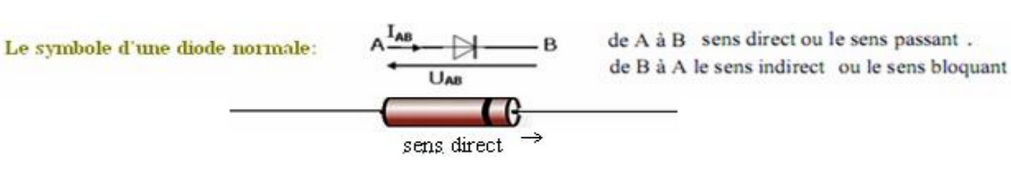
\includegraphics[width=0.7\textwidth]{./img/Diode_E.png}
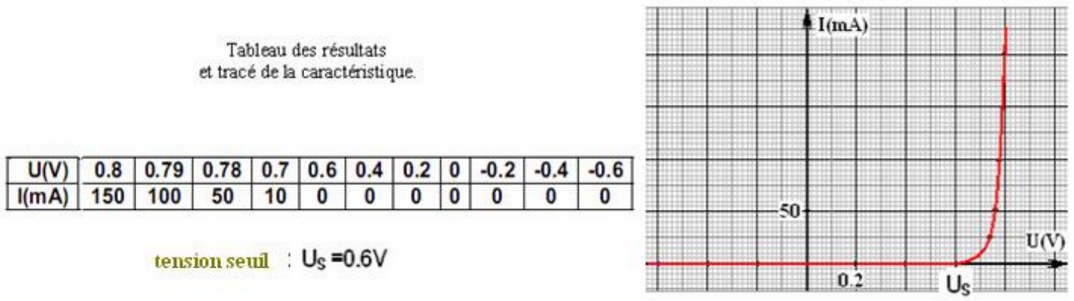
\includegraphics[width=0.7\textwidth]{./img/carca_diode_e.png}

\end{center}

\begin{tcolorbox}{conclusion}
-La caractéristique passe par O , donc la diode est un dipôle passif.

  -Pour $U_{AB}\leq U_S$ , la diode ne laisse pas passer le courant électrique .

  -la diode laisse pas passer le courant électrique . Pour $U_{AB} >= U_S$

 La diode est un dipôle passif non symétrique et non linéaire ,elle ne laisse passer le courant que
dans le sens direct si la tension à ses bornes est supérieure ou égale à la tension seuil.
\end{tcolorbox}

\subsection{Caractéristique d'une diode Zener: }
Une diode Zener est un assemblage de deux semi-conducteurs:
\begin{center}
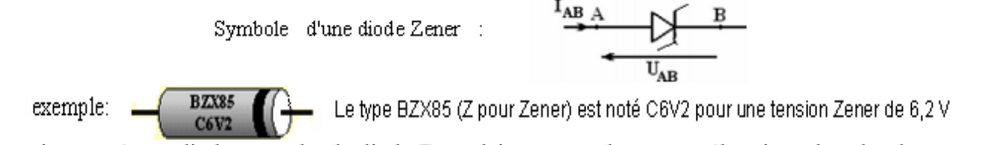
\includegraphics[width=0.5\textwidth]{./img/Ziner_diode.png}
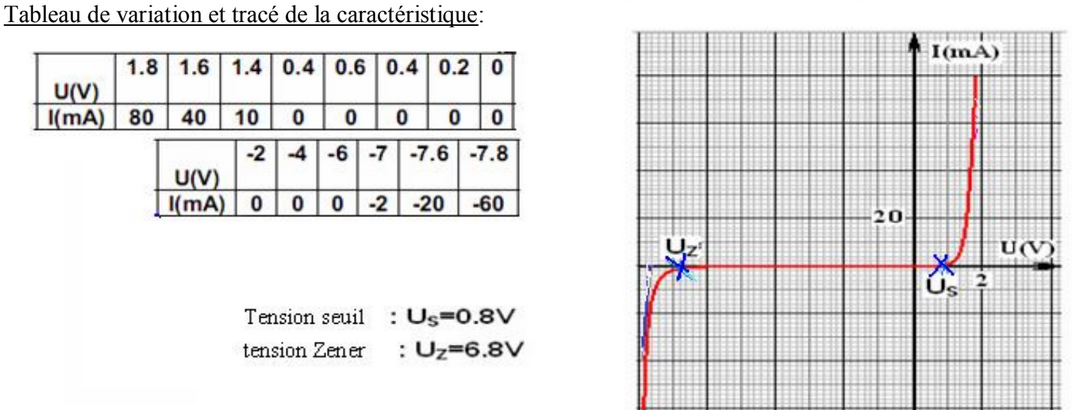
\includegraphics[width=0.7\textwidth]{./img/Zener_carct.png}
\end{center}

Contrairement à une diode normale , la diode Zener laisse passer le courant électrique dans les deux sens.



\begin{tcolorbox}
La caractéristique passe par O , donc la diode Zener est un dipôle passif.

  La caractéristique est asymétrique donc les bornes de la diode Zener ne jouent pas le même rôle..

  Dans le sens direct la diode Zener se comporte comme une diode normale..

  Dans le sens inverse la diode Zener laisse passer le courant électrique si la tension à ses bonnes est supérieure à
la tension Zener.
\end{tcolorbox}

\subsection{Caractéristique d'une varistance ou VDR:}
La varistance VRD est un résistor  dont la résistance dépend de la tension 

VRD provient de l'expression anglais <Voltage depend resistor>.



\begin{center}
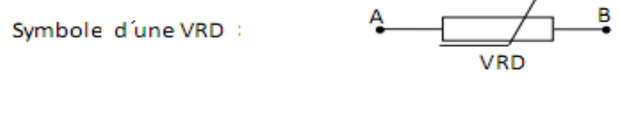
\includegraphics[width=0.2\textwidth]{./img/VDR.png}
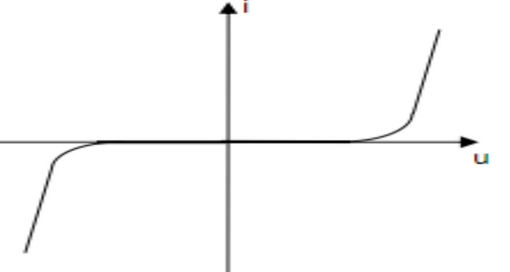
\includegraphics[width=0.2\textwidth]{./img/VDR_carca.png}

\end{center}
La caractéristique d'une VDR est symétrique et non linéaire donc ses deux bornes jouent le même rôle.


\subsection {Caractéristique d'une thermistance CTN ou CTP: }
Les thermistances sont des résistances qui ont la propriété de varier avec la température. On en distingue deux

types : les thermistances à coefficient de température positif (CTP) et les thermistances à coefficient de
température négatif (CTN).
\begin{center}
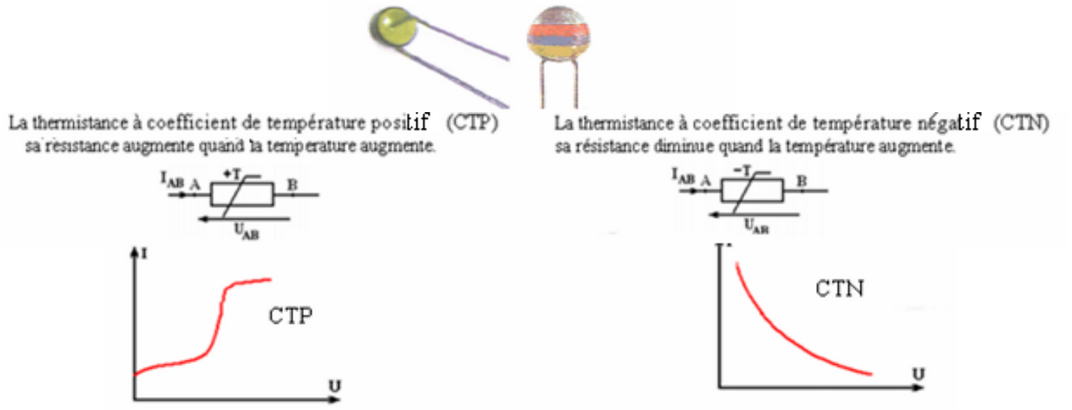
\includegraphics[width=0.7\textwidth]{./img/CTN_CTP.png}

\end{center}

Quand la température augmente la valeur de la résistance de la CTP augmente et celle de la CTN diminue.
\subsection{Caractéristique de la photorésistance (LDR): }
La photorésistance est un dipôle dont la résistance dépend de la l'éclairement qu'il reçoit. 
\begin{center}
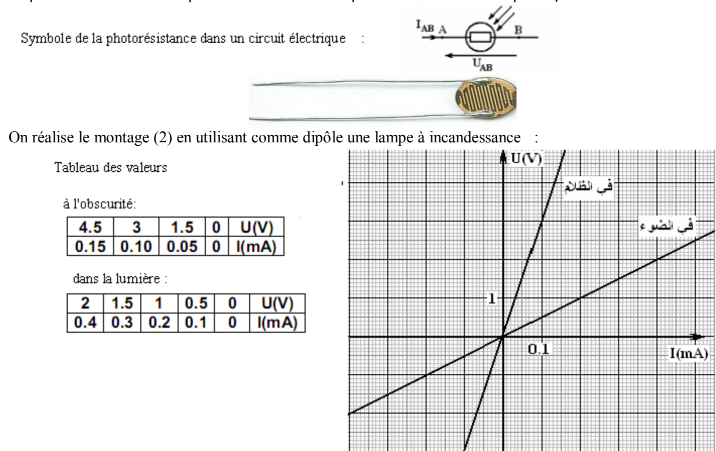
\includegraphics[width=0.7\textwidth]{./img/LDR.png}

\end{center}
\subsection{Caractéristique d'une diode électroluminescente (LED):}
Une diode électroluminescente est un dipôle qui se comporte comme une diode normale et qui est capable d’émettre
la lumière lorsqu'elle parcouru pa un courant électrique.
\begin{center}
  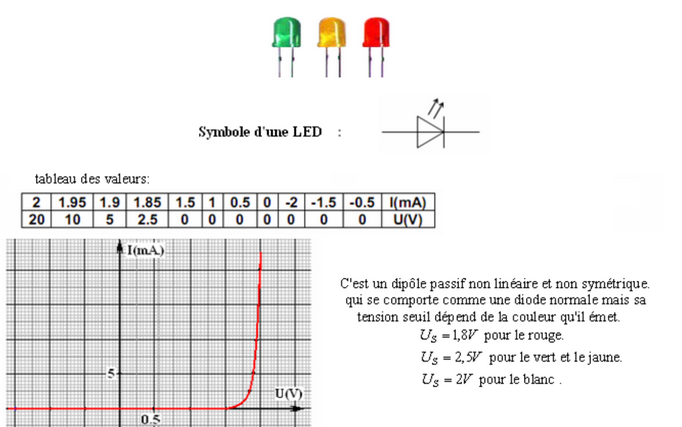
\includegraphics[width=0.7\textwidth]{./img/Led_teh.png}

\end{center}
\end{document}
